\section{Gaussian Process Regression Model}\label{GPR}

GP models can be applied as probabilistic models to regression problems.  Here we will use the GP model to generalise a grid of stellar models to a continuous and probabilistic function that maps inputs (i.e., initial mass, chemical composition, etc.) to observable quantities (i.e., effective temperature, surface gravity, radius, etc.).  We aim to use the GP model as a non-parametric emulator, that is emulating the comparatively slow calls to models of stellar evolution. 
%
We adopted the a tool package named \textsc{GPyTorch}, which is a GP framework developed by \citep{gardner2018gpytorch}. GPyTorch is a Gaussian process library implemented using PyTorch. We adopted this tool package because it provides significant GPU acceleration, state-of-the-art implementations of the latest algorithmic advances for scalability and flexibility, and easy integration with deep learning frameworks. Source codes and detailed introductions could be found on \url{https://gpytorch.ai} 


\subsection{Gaussian Process Application}

We start with a grid of stellar models containing $N$ models with a label we want to learn, for example model effective temperature, which we will denote with the general symbol $\bf y$, and a set of input labels $\bf X$ (e.g., mass, age, and metallicity).  We can use a GP to make predictions of the effective temperature (or $y$) for additional input values given by $\bf X_{\star}$.  The vector $\bf y$ is arranged ${\bf y} = \left(y_{i}, ... ,y_{N} \right)^{T}$ where the subscript label references the stellar model.  The input labels are arranged into a $N \times D$ matrix where $D$ is the number of input dimensions (e.g., $D=3$ for mass, age, and metallicity) so that ${\bf X} = ({\bf x}_{1}, ..., {\bf x}_{N})^{T}$ where ${\bf x_{i}} = (x_{1, i}, ..., x_{D, i})^{T}$.  The matrix of additional inputs $\bf X_{\star}$ has the same form as $\bf X$ but size $N_{\star} \times D$.

Rasmussen and Williams (!REF!), from which our description below is based, define a GP as a collection of random variables, where any finite number of which have a joint Gaussian distribution.  In general terms, GP's may be written as
\begin{equation}
y({\bf x}) \sim \mathcal{GP}\left( m({\bf x}), {\bf \Sigma}\right),
\end{equation}
where $m({\bf x})$ is some mean function, and ${\bf \Sigma}$ is some covariance matrix.  The mean function controls the deterministic part of the regression and the covariance controls the stochastic part.  The mean function defined here could be any deterministic function and we will label the additional parameters, or hyperparameters, $\phi$.  Each element of the covariance matrix is defined by the covariance function or {\it kernel function} $k$ which has hyperparameters $\theta$ and is given by,
\begin{equation}
{\bf \Sigma}_{n, m} = k({\bf x}_{n}, {\bf x}_{m}),
\end{equation}
where the inputs ${\bf x}_{i}$ are $D$-dimensional vectors and the output is a scalar covariance.

As a GP is a collection of random variables, where any finite number of which have a joint Gaussian distribution, the joint probability of our data $\bf y$ is
\begin{equation}
p({\bf y} | {\bf X, \phi, \theta}) = \mathcal{N}(m({\bf X}), {\bf \Sigma}).
\end{equation}
If we want to obtain predictive distributions for the output $\bf y_{\star}$ given the inputs $\bf X_{\star}$ the joint probability distribution of $\bf y$ and $\bf y_{\star}$ is Gaussian and given by
\begin{equation}
p \left( \begin{bmatrix} {\bf y} \\ {\bf y_{\star}} \end{bmatrix} \right) = \mathcal{N} \left( \begin{bmatrix} {\bf X} \\ {\bf X_{\star}} \end{bmatrix} , \begin{bmatrix} {\bf \Sigma} & {\bf K_{\star} }\\ {\bf K_{\star}}^{T} & {\bf K_{\star \star}} \end{bmatrix}  \right), 
\end{equation}
where the covariance matrices $\bf \Sigma$ and $\bf K$ are computed using the kernel function so that
\begin{equation}
{\bf \Sigma}_{n, m} = k({\bf X}_{n}, \, {\bf X}_{m}),
\end{equation}
which is an $N \times N$ matrix.
\begin{equation}
{\bf K}_{\star \, n, m} = k({\bf X}_{n}, \, { \bf X}_{\star \, m}),
\end{equation}
which is an $N \times N_{\star}$ matrix, and finally
\begin{equation}
{\bf K}_{\star \star \, n, m} = k({\bf X}_{\star \, n},  {\bf X}_{\star \,m}),
\end{equation}
which is an $N_{\star} \times N_{\star}$ matrix.
The predictions of $\bf y_{\star}$ are again a Gaussian distribution so that,
\begin{equation}
{\bf y}_{\star} \sim \mathcal{N}(\bf \hat{y}_{\star}, \, \bf C),
\label{eq:pred}
\end{equation}
where 
\begin{equation}
{\bf \hat{y}}_{\star} = m({\bf X}_{\star}) + {\bf K}_{\star}^{T} \, {\bf \Sigma}^{-1} \, ({\bf y} - m(\bf X)),
\end{equation}
and 
\begin{equation}
{\bf C} = {\bf K}_{\star \star} - {\bf K}_{\star}^{T} \, {\bf \Sigma}^{-1} \, {\bf K_{\star}}.
\end{equation}

At point we can make predictions on model properties given a grid of stellar models using equation \ref{eq:pred}.  But these predictions will be poor unless we select sensible values for the form and hyperparameters of the mean function and covariance function.  In the following section we detail a number of kernel functions that will be tested against the data.  We will then discuss the method for determining the values of the hyperparameters to be used.

\subsection{GP Model Inputs and Outputs}
We aim to derive stellar parameters based on fundamental inputs of the model grid. As mentioned in Section~\ref{sec:grid}, our model grid has five independent fundamental inputs, says, mass, initial metallicity, initial helium fraction, mixing-length parameter, and the age.
Among them, the age ranges of individual evolutionary tracks significantly vary with the mass and other model inputs and hence are not ideal as the GP model inputs. The fractional age is an option. However, the evolution of global parameters around the 'hook' and the turn-off point performs sharp changes within a short time scale as shown in the left panel of Figure~\ref{fig:eep}. The sharp features are hard to learn and hence poorly predicted by GP models. To overcome this issue, we followed MIST(add ref here) and introduce an Equivalent Evolutionary Phase ($EEP$ here after) to replace the age as fundamental inputs. Note that our definition of $EEP$ is different from MIST. 
%
On each evolutionary track, we compute the displacement of a evolving step $n$ on the  $T_{\rm eff} - \log g$ as 
\begin{equation}\label{eq:disp}
\delta d_{n} = ((T_{\rm eff, n-1} - T_{\rm eff, n}) ^{2} + (\log g _{n} - \log g_{n-1})^{2}))^{f},
\end{equation}
and the total displacement of a data point $n$ 
\begin{equation}
d_{n} = \sum_{i = 0}^{i = n} \delta d_{i} .
\end{equation}
The normalised $d_{n}$ (to a 0 --1 range) is defined as $EEP$. On the same evolutionary track, $EEP$ equals to 0 at the ZAMS and 1 at $\log$ = 3.6 $dex$. The factor $f$ in Eq. \ref{eq:disp} is for modulating $EEP$ to avoid large gap in the parameter space, and we found that $f$ = 0.18 gives the best data distribution. {\bf add figures in appendix}
%
We illustrated two GPR models with the fractional age and $EEP$ as inputs in Figure~\ref{fig:selection_of_t} which shows the advantages of EEP.
It can be seen in the top graph that the effective temperature evolution presents a sharp hump around 0.7 (the hook) and quickly drops in the last 10\% lifetime. Using $EEP$ instead of fractional age significantly smoothes the curve and make it easer to fit. As we compare in Figure~\ref{fig:eep}, using EEP instead of fractional age gives a much smoother change at the hook and turn-off points. 

We summary our selections of GPR model inputs and outputs as below. 
\begin{itemize}
\item GPR model inputs and their dynamic ranges:
\item[] Mass ($M$ = 0.8 -- 1.2$M_{\odot}$)
\item[] Equivalent Evolutionary Phase ($EEP$ = 0 -- 1)
\item[] Initial metallicity ([Fe/H]$_{\rm init}$ =  -0.5 -- 0.5)
\item[] Initial helium fraction ($Y_{\rm init}$ = 0.24 -- 0.32)
\item[] Mixing-length parameter ($\alpha_{\rm MLT}$ = 1.7 -- 2.5)
\item GPR model outputs: 
\item[] Effective temperature ($T_{\rm eff}$) 
\item[] Surface gravity ($\log g$)
\item[] Radius ($R$)
\item[] The large spacing ($\Delta\nu$)  
\item[] Surface metallicity ([Fe/H]$_{\rm surf}$)
\item[] Age ($\tau$)
\end{itemize}
Thus, our GPR model can be described as 
\begin{equation}\label{gprmodel}
{\rm Outputs} = f(M, t', ({\rm Fe/H})_{\rm init}, Y_{\rm init}, \alpha_{\rm MLT}). 
\end{equation}

\begin{figure*}
        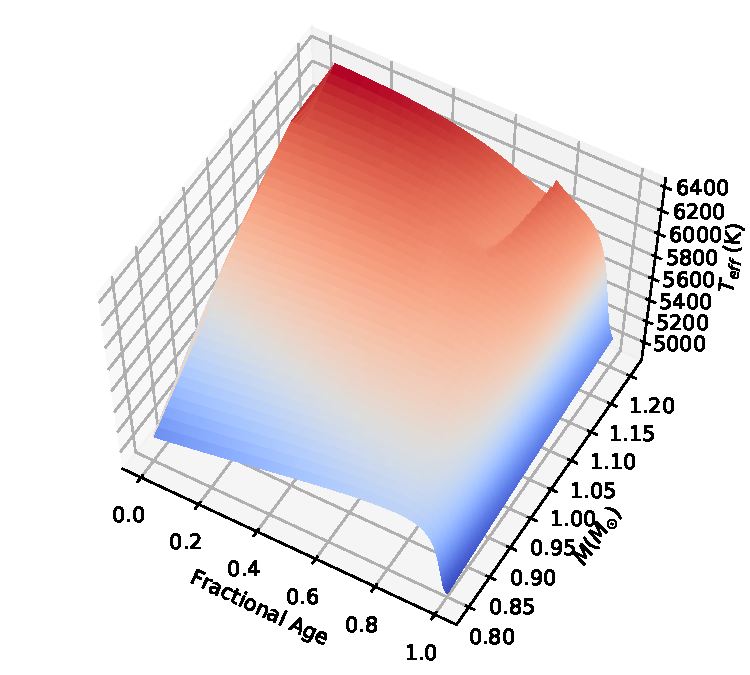
\includegraphics[width=1.\columnwidth]{2d_fage_data.pdf}
	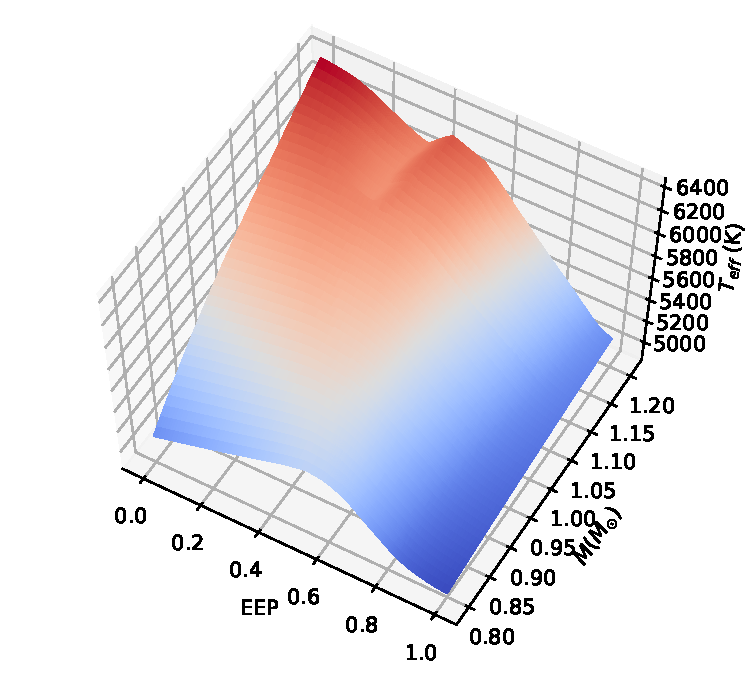
\includegraphics[width=1.\columnwidth]{2d_EEP_data.pdf}
     \caption{Surface plots of effective temperature as a function of fractional age (left) and EEP(right). It can be seen that using EEP instead of fractional age as the input gives much smoother features at the hook and turn-off points.}
    \label{fig:eep}
\end{figure*}

\subsection{Training Procedure}\label{workflow}
  
\subsubsection{Data Selection}

We have three types of data for training, validating, and testing GP models. The model grid is apparently the training data and the off-grid models are divided into validating and testing datasets by half to half. Note that validating and testing data are not on same evolutionary tracks so they do not share any information. Validating dataset is for validating the GP model in the training process and is mainly used for early stopping, which is a form of regularisation for avoiding overfitting. We choose off-grid models but not on-grid models as validating data because the grid is equally spaced. Without additional information between grid points, an optimiser could either use a smooth function or a periodic function to fit the data and find no obvious differences in the likelihood. We describe how we use validating data in Section \ref{sec:training}. Lastly, testing dataset is independent on the training process and used for evaluating the final GP models. 

Because the computational and memory complexity exponentially increase with the number of data involved in the Gaussian Process, only a subset of the model grid can be adopted. Moreover, the data density are not same at different evolutionary stages due to the \textsc{MESA} step-control strategy: stellar models are dense at the main-sequence and the red-giant phases but quite sparse on subgiant stage. The sampling method is hence critical to the performance of GP models. Firstly, we want the data to uniformly cover the parameter space for the best efficiency. Secondly, we need to highly weight models at phases where sharp changes present, e.g., models around the hook and turn-off points.   
We tested a few methods and found that using the displacement ($\delta d_{n}$) defined in Eq.~\ref{eq:disp} to weight sampling meets the above two requirements. 

\subsubsection{Training, Validating, and Testing GP Models}\label{sec:training}

We train GP models as a regression problem. We develop our training process based on two standard examples (Simple GP Regression and Stochastic Variational GP Regression) in the \textsc{Gpytorch} packages. We test different approaches to determine the training method. Details are described and discussed in the next Section. In the training process, we validate the GP model in every iteration and save it as the best model when the validation index decreases. The training terminate when the validating results stop improving for 300 iterations. Lastly, the best GP model is tested with the testing dataset.

Here we discuss the method for validating and testing a GP model. We do not use popular methods, such like RME because the GP model performances are not uniform across the whole parameter space due to different evolutionary features. We illustrate this in Figure \ref{fig:2dtest} with a 2D GP model for $T_{\rm eff}$. As it can be seen that, the function for the hook area ($M \geq 1.05 M_{\odot}$ and $EEP \leq 0.7$) is more complex than that for other smooth regions. The evolutionary features in this particular area are hence relatively difficult to learn by the GP model, leading to obvious different accuracy levels (as shown in the bottom graph).
%
For other output parameters, surface gravity and radius are similar to the case of effective temperature: obviously differences between the 'hook' and other area. The evolutionary feature of surface metallicity is not significantly affected by the hook, but the testing errors of its GP model are obviously higher at the early subgiant phase for high-mass tracks. This is because high-mass tracks maintain shallow convective envelope and hence have strong diffusion effect during the main-sequence stage.  Their surface metallicities at then end of the main-sequence are generally much lower than the initial value. When high-mass models evolve to the early subgiant phase, the quick expansion of the surface convective envelope brings back the settling heavy elements to the surface, resulting in a sharp raise of the surface metallicity.  When there is a sub-region in the parameter space where GP models always peforme worse than other areas, a RME value is not suitable. We hence need a validation method that reflects the general accuracy of a GP model as well as its performance in these particular regions.   
%
To find a proper method for validation, we examine the error distribution as shown at the bottom of Figure \ref{fig:2dtest}. For the case of effective temperature, errors of most loss-mass data follows a Gaussian distribution. Data in the hood-affected regions is $\sim10\%$ of the total sample. This is a small proportion hence does not significantly affect the main feature but form long tails on both sides.  
%
For validating the general accuracy, a standard deviation is suitable. The long tail could be quantity by two cumulative values: one at 95\% indicates the median error of the these values, the other at 99.7\% to describe the scatter. Thus, we use the sum of three cumulative values (at 68\%, 95\%, and 99.7\%) of absolute validation errors as an error index to qualify a GP model in validating and testing progresses. For the case in Figure \ref{fig:2dtest}, cumulative values at 68\%, 95\%, and 99.7\% are 1.07, 4.86, and 11.05$K$, which give an error index equals to 16.98. 

\begin{figure}
	% To include a figure from a file named example.*
	% Allowable file formats are eps or ps if compiling using latex
	% or pdf, png, jpg if compiling using pdflatex
	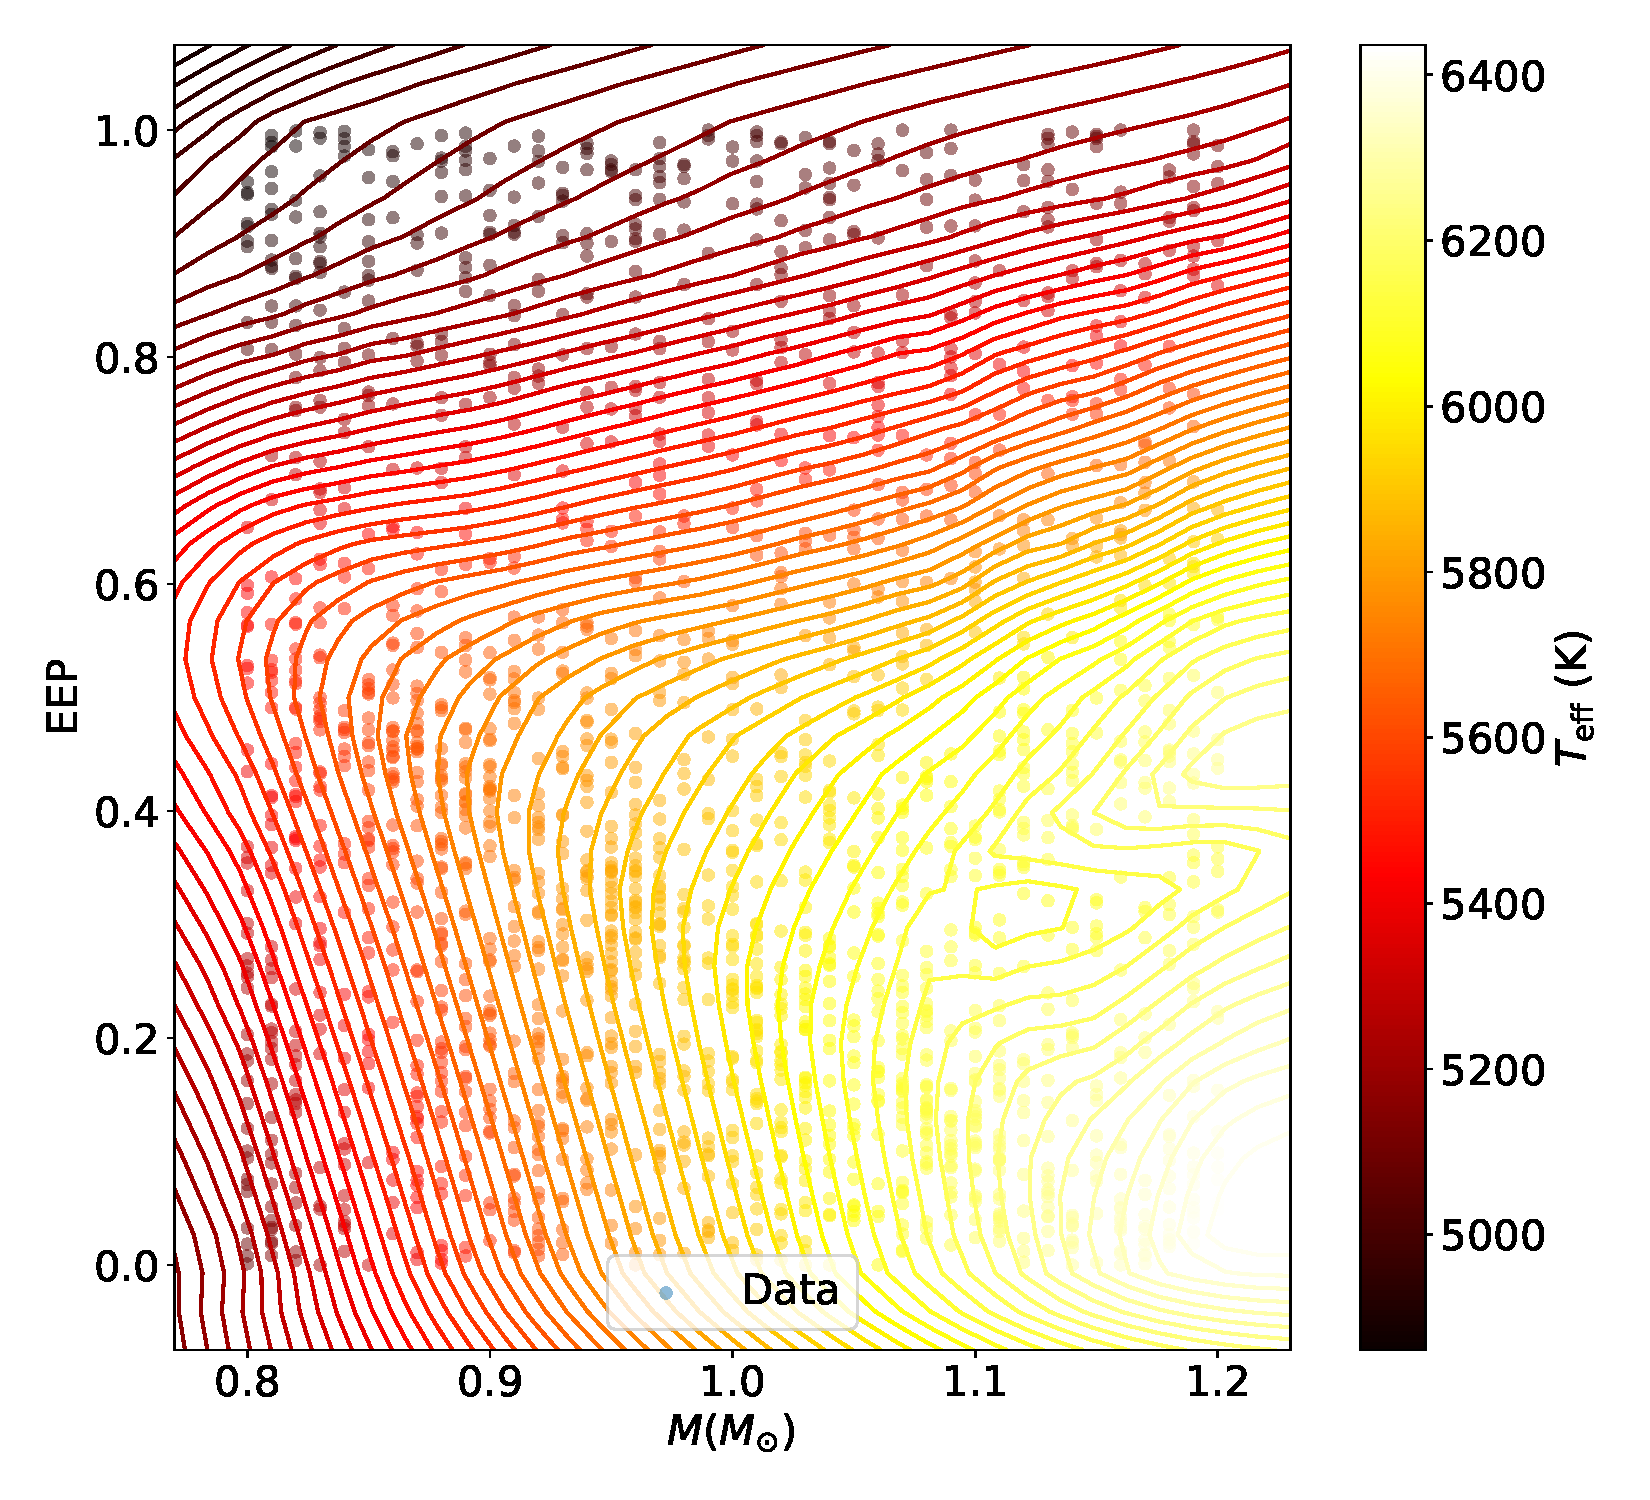
\includegraphics[width=1.0\columnwidth]{2d_GPmodel_function.pdf}
	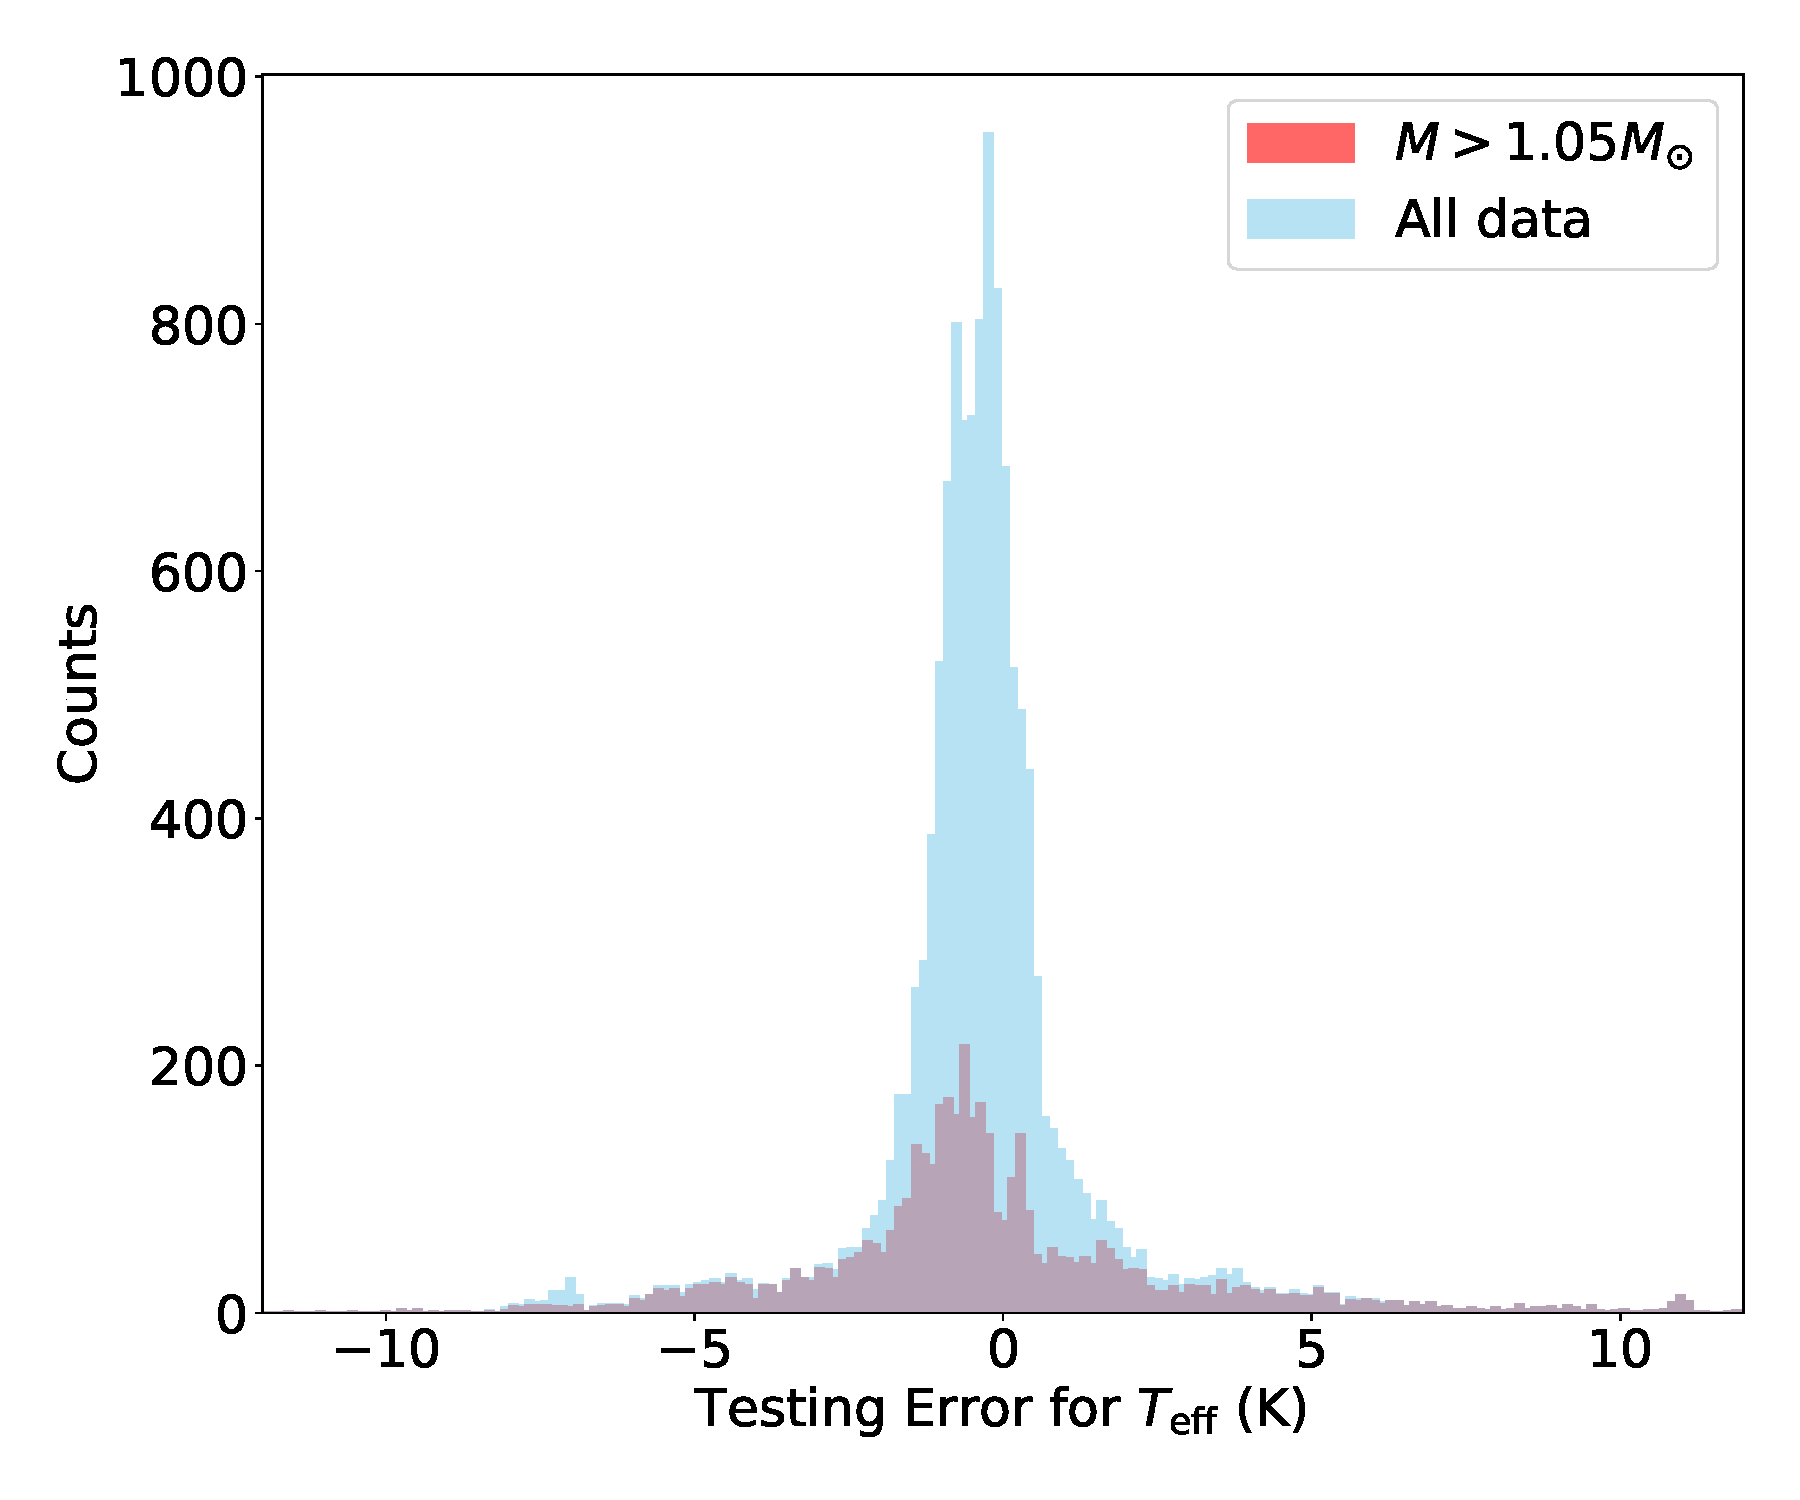
\includegraphics[width=1.0\columnwidth]{2d_testing_hist_effective_T.pdf}	
    \caption{Top: The 2D GP model for $T_{\rm eff}$. Bottom: probability distributions of validating errors of the GP model. }  
    \label{fig:2dtest}
\end{figure}


\subsection{Primary Tests and Settings of Training}

Before training the grid, we need to set up the GP model including mean function, kernel, likelihood function, loss function, and the optimiser. As there are not many relevant studies, we test how different options affects the GP models and decide which to use. These primary tests are done with simple 2-demission (2D) GP models, which have two inputs: $M$ and $EEP$ and can be described as $p = f(M, EEP)$. 
%
Data for training 2D models (2D data here after) are selected  from the primary grid with fixed [Fe/H]$_{\rm init}$ (0.0), $Y_{\rm init}$ (0.28), and $\alpha_{\rm MLT}$ (2.1). The training dataset contents 41 evolutionary track and 24,257 data points.
%
We also computed 44 evolutionary tracks with same input [Fe/H]$_{\rm init}$, $Y_{\rm init}$, and $\alpha_{\rm MLT}$ but random $M$ for validating and testing the GP models. 

The 2D model can be trained with the Exact GP approach because the training data size is approximate 20,000. We start with the \textsc{Simple GP Regression} example (\url{https://docs.gpytorch.ai/en/stable/examples/01_Exact_GPs/Simple_GP_Regression.html})  to develop our training script.

\subsubsection{Mean Function}

We start with testing different mean functions. As demonstrated in Figure~\ref{fig:eep}, the map between model inputs and outputs show various of features in different regions of the parameter space: models with relatively high mass have complex curvatures around the hook and the turn-off point while other models follow smooth functions. Although the GP model does not significantly affected by the choice of the mean function due to the flexibility of kernels, we find that a simple mean function (constant or linear) leads to a long time for training and a significant increase of the complexity of kernels. We hence applied a more complex mean function which is flexible enough to map smooth as well as curved features. A Neural Network is well suitable. To cover higher-demissions GP model, we adopt an architecture includes 6 hidden layers and 128 nodes per layer. All layers apply the linear transformation to the incoming data. We apply the element-wise function (Elu) because it give relatively smooth mean functions. (add ref for NN and Elu)

\subsubsection{Likelihood and Loss Function}

We then test for the likelihood and loss function. Our training object is a theoretical model grid, there is hence no observed uncertainty for each data point. However, a tiny random uncertainty exists due to the approximations in the \textsc{MESA} numerical method. The noise model can be assumed as a Gaussian function with a very small deviation. We hence applied the standard Gaussian Likelihood function in \textsc{GPyTorch}. 
%   
A Likelihood  specifies the mapping from latent function values $f(X)$ to observed labels $y$.
We adopt the the standard likelihood for regression which assumes a standard homoskedastic noise model whose conditional distribution is
\begin{equation}\label{eq:likelihood}
p(y|f(x)) = f + \epsilon, \epsilon \sim \mathcal{N}(0, \sigma^{2}),
\end{equation}
where $\sigma$ is a noise parameter. 
%
Given the random uncertainty is small, we set up a small and fixed noise parameter and run a few tests. However, we found that it makes the GP models hard to converge and sometimes lead to obvious overfitting (poor behaviour between grid). When we set up this noise parameter free and start with a large initial value, it reduces to a small number anyway in the training progress because it is data-driven. For these reasons, we decide not put strict constraint for or prioritise this noise parameter and let the data determine. In practice, we set up a loose upper limit ($\sigma$  < 0.1) for the noise parameter. However, it should be note that a GP model with a larger noise parameter can not be a proper description for the training data even if it gives good validating or testing errors. Because of this, we only use GP model with a noise parameter $\lesssim 10^{-4}$.   
The the loss function is simply the exact marginal log likelihood.

\subsubsection{Optimiser}

With a Neural Network mean function and Gaussion likelihood function, we then run tests to decide the optimiser. We mainly compare two optimisers named SGD and Adam. Here SGD refers to Stochastic Gradient Descent, and Adam is a combination of the advantages of two other extensions of stochastic gradient descent, specifically, Adaptive Gradient Algorithm and Root Mean Square Propagation. 
%
The SGD optimiser in the \textsc{Troch} packages involved the formula from \citet{sutskever2013importance}, which makes it possible to train using stochastic gradient descent with momentum uses a well-designed random initialisation and a particular type of slowly increasing schedule for the momentum parameter. The application of momentum in SGD could improve its efficiency and make it less likely to stuck in local minimums. On the other hand, the Adam optimiser includes the \textsc{AMSGrad} variant developed by \citet{47409} to improve its weakness in the convergence to an optimal solution. With these new developments, the two optimisers give very similar results. We finally choose Adam because it works more efficiently and stable than the SGD.  
%
We adaptive learning rate instead of a fixed value. All training starts with a learning rate of 0.01 and decreases by a factor of 2 when the loss value stop reducing in the previous 100 iterations.    

\subsubsection{Early stopping}
We set up an early stoping method to determine when to terminate the training progress based on the validation index introduced in Section~\ref{sec:training}. In our training progress, we validate the GP model every iteration and save the current model if the validating results is by far the best. When an optimal solution is found, the validating errors stop decreasing and start increasing at some point when overfiiting occurs. To be efficient and prevent overfitting, we terminate the training progress when the validating index does not decrease in the previous 300 iterations. The last saved GP model will be adopted.   

\subsubsection{GP kernels}

With the above settings, we lastly test for selecting the best kernel for this work. We involved four basic kernels the tests as listed below:
\begin{itemize}
\item RBF: Radial Basis Function kernel (also known as squared exponential kernel)
\item RQ: Rational Quadratic Kernel (equivalent to adding together many RBF kernels with different lengthscales)
\item Mat12: Matern 1/2 kernel (equivalent to the Exponential Kernel)
\item Mat32: Matern 3/2 kernel 
\end{itemize}
We applied each basic kernel and numbers of combinations (RBF + Mat21, RQ + Mat21, Mat32 + Mat21, RBF + Mat32, RQ + Mat32) to train the 2D GP models. Among these kernels, the combined one RBF+Mat21 give the best fit to the training data, however, it does not give the best predictions for the validating and testing data (off-grid).  On the other hand, the GP model with the Mat32 kernel gives good (but not the best) fit for the training data, but the best accuracies for validating and the testing data. 
%
Comparing between the two kernels, the RBF+Mat12 Kernel is a combination of a smooth and a spiky kernel, which offers enough flexibility fit most features in the training data. However, the spiky function well fitting the sharp features will be applied in the nearby off-grid regions and this causes poor predictions. 
%
The smoothness of Mat32 is somewhere between a spiky (Mat21) and a smooth kernel (RBF). For the sharp changes, it gives a relatively smooth function compared with the Mat21 kernel and hence perform a good balance between on- and off-grid data. 
%
In the final models, we hence adopted Mat32 kernels for all trainings.  

 \subsection{Strategy for Large sample}

The model grid we aim to train contents about 10,000,000 data points, which is much more than the upper limit of data size of the Exact GP (20,000). We hence consider other GP approaches. Our tests for the large-sample strategy are carried out with a 3-demission (3D) GP model, which have three fundamental inputs: $M$ and $EEP$ and  [Fe/H]$_{\rm init}$. The 3D model can be described as  ($p = f(M, EEP, {\rm [Fe/H]_{init}})$). 
Data for training 3D models (3D data hereafter) are from the primary grid with fixed $Y_{\rm init}$ (0.28), and $\alpha_{\rm MLT}$ (2.1). The training sample include 562 tracks and $\sim$ 300,000 data points. 
%
For validating and testing purposes, we computed 174 evolutionary tracks with the same input $Y_{\rm init}$, and $\alpha_{\rm MLT}$ but random $M$ and [Fe/H]$_{\rm init}$ within grid ranges. 


We first consider the Stochastic Variational GP (SVGP) with \textsc{GPyTorch ApproximateGP} module and test with the example on \url{https://docs.gpytorch.ai/en/v1.1.1/examples/04_Variational_and_Approximate_GPs/SVGP_Regression_CUDA.html}. SVGP is an approximate scheme rely on the use of a series of inducing points which can be selected in the parameter space. It trains using minibatches on the training dataset and build up kernels on the inducing numbers. Underline principles and detailed descriptions of this approach can be found in \citet{hensman2015scalable}. The advantage of SVGP is the large capacity of sample size, however, the kernel complexities is still limited by the amount of inducing numbers. If SVGP uses inducing numbers as many as the training data of the Excat GP, better prediction accuracy will be expected because more information is given. Unfortunately, the the GPU memory is limited. When more training data is loaded, the inducing number for SVGP can not go up to 20,000 in our training. On the same GPU, a SVGP model is able to use up to10,000 inducing number when 100,000 training data is loaded. This is to say, although a SVGP model involves more data but sacrifices the kernel complicity compared with an Exact GP model. 
%
Our comparison between a SVGP model (with 10,000 inducing number with 100,000 training data) 
and an Exact GP model (with 20,000 training data) shows that the SVGP framework does not improve the GP model performance. 
%
For instance, the testing errors of $T_{\rm eff}$ at 68\%, 95\%, and 99.7\% are 2.0, 5.8, and 15.7 $K$ (error index = 23.5$K$)  for Exact GP model and 2.2, 6.8, and 15.1 $(error index = 24.1)$ for the SVGP model. 


We then investigate another approach designed for the large dataset named Structured Kernel Interpolation (SKI GP). SKI GP was introduced by \citet{wilson2015kernel}. It produces kernel approximations for fast computations through kernel interpolation and is a great way to scale a GP up to very large datasets (100,000+ data points). We follow the example on \url{https://docs.gpytorch.ai/en/stable/examples/02_Scalable_Exact_GPs/KISSGP_Regression.html} to develop our script. We run a few tests to train a 3D SKI GP model with 100, 000 training data. Compare with the Exact GP and SVGP, its testing errors of $T_{\rm eff}$ are slightly improved to 2.0, 6.1, and 14.8 $K$ (error index = 22.9 $K$). However, the further test on the 5-demission data is not ideal: a SKI GP model with 100,000 training data performs much worse than an Exact GP model with 20,000 training data. The poor behaviour of the 5D model consist with what has been discussed in \citet{wilson2015kernel}. The method won’t scale to data with high dimensions, since the cost of creating the grid grows exponentially in the amount of data. We attempt to make some additional approximations with the \textsc{GpyTorch AdditiveStructureKernel} module. It makes the base kernel to act as one-dimension kernels on each data dimension. and the final kernel matrix will be a sum of these 1D kernel matrices. Although the testing errors are improved but still worse than the simple Exact model. Thus, the SKI GP framework is also not ideal for our goal.   

 \begin{figure}
	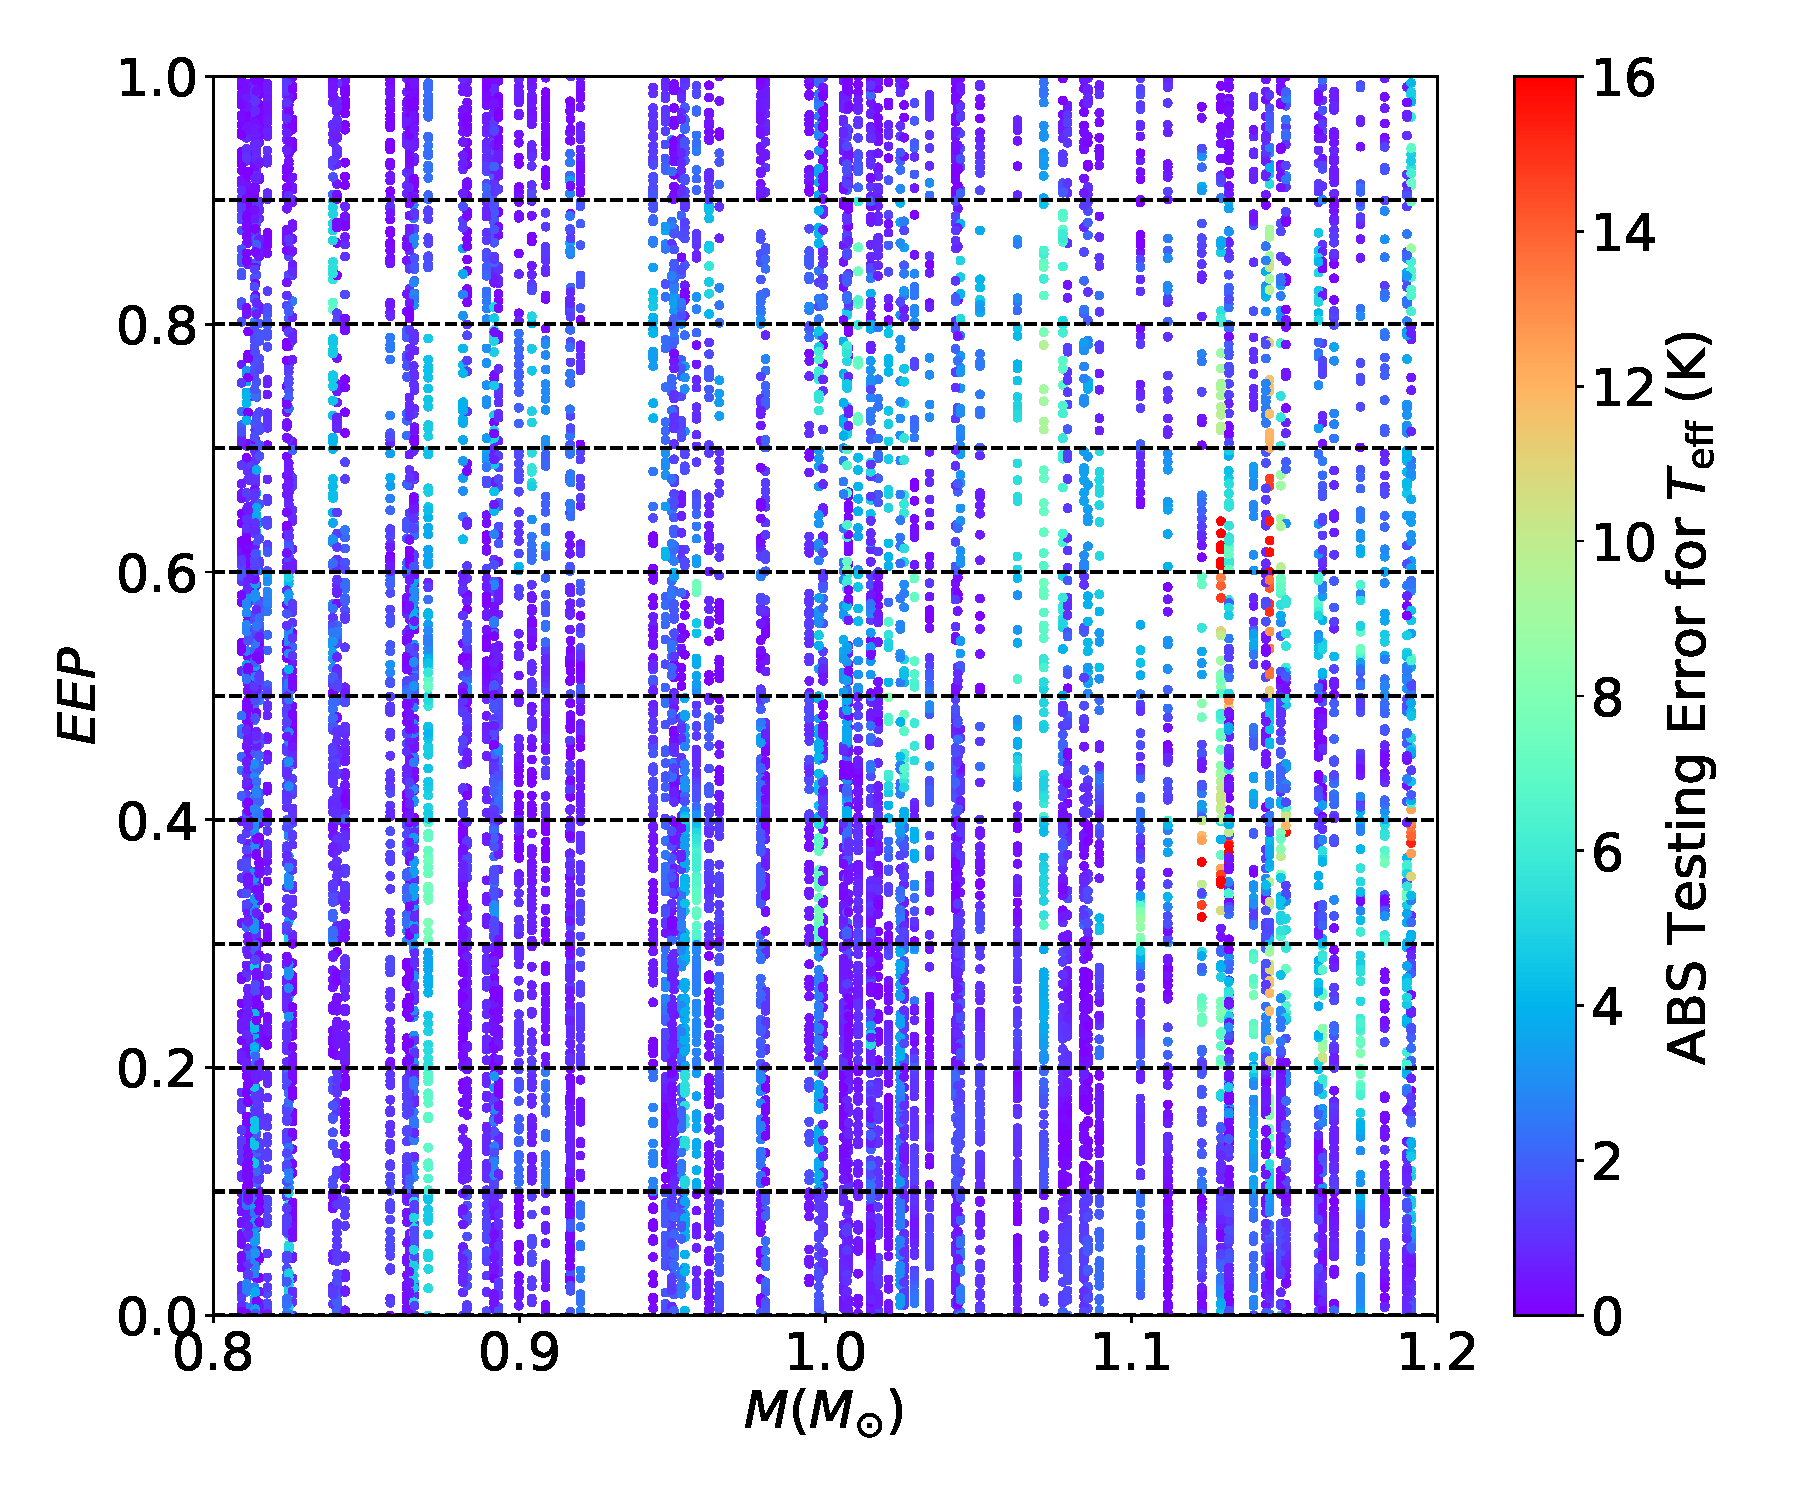
\includegraphics[width=1.0\columnwidth]{3d-testing_teff-10sections.pdf}
	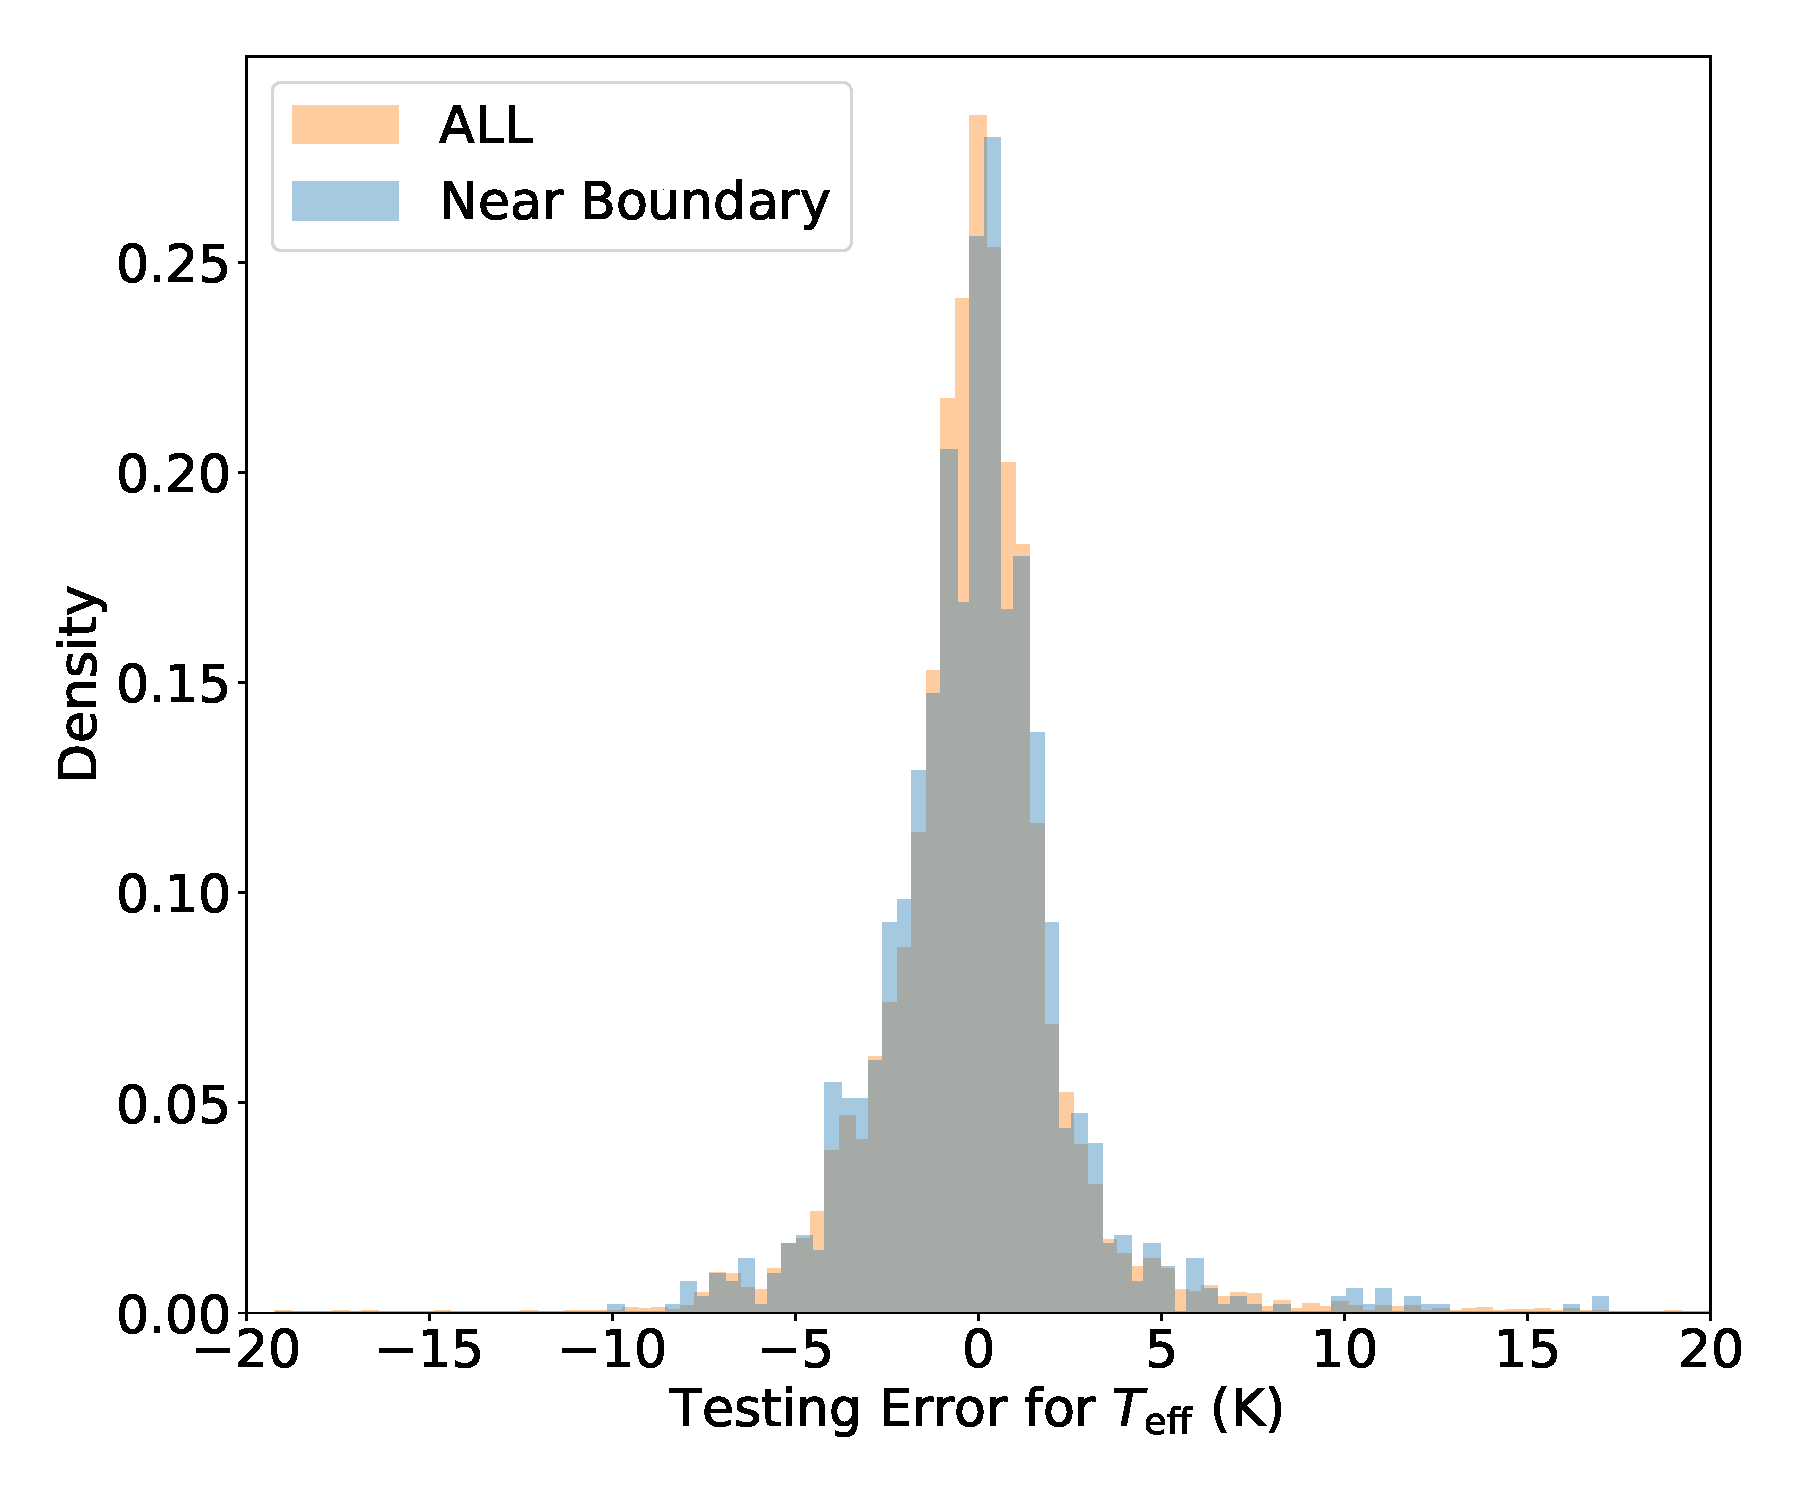
\includegraphics[width=1.0\columnwidth]{3d-testing_teff-hist-10sections.pdf}	
    \caption{Top: Testing errors of 3D GP model for $T_{\rm eff}$ on the $M -- EEP$ diagram. Dashes indicates section boundaries. Bottom: examination of the edge effects of the section scenario. Probability distributions of testing errors of all testing data and those near the boundary ($\pm$0.01 EEP) in the upper graph are compared.  As it can be seen, testing errors do not raise around the boundary. }  
    \label{fig:3dtest}
\end{figure}


As mentioned above, the GPU memory captivity limits the actual number of data that induce the kernel and hence the accuracy level.  
This limit become critical for high-demission cases, because the parameter space exponentially increases with model demission and hence GP model accuracy inevitable declines. Thus, a simple way of improving GP models is using more data to induce kernels. 
%
For this reason, we break the grid into a number of sections and train GP models for each section separately. With the same 20,000 training data for a single GP model, 10 sections means 10 times of the data are used to describe the grid. 
%
The downside of this section scenario is obvious: there will not be one GP model that maps the whole grid. However, as long as the goal of this work is augmenting a model grid but not deriving a universal function for stellar evolutions, this scenario is suitable. 

Here we test how this approach works for the 3D data. We divide the dataset into 10 equal segments by $EEP$. We train one Exact GP model with 20,000 training data for each output parameter in each section. We then use the same testing dataset as used above to quantify predictions for the five outputs, and the error index are averagely improved by around 10\%. For instance, the error index of $T_{\rm eff}$ decreases from 23.5 to 21.6 (1.7/5.0/14.9 $K$ at 68/95/99.7\%). 
%

The section scenario method gives a better accuracy as expected, but there is a major concern about the edge effects at the boundary between sections. If the model works significantly poor at the boundary between sections, it will be difficult to map the systematic errors across the whole parameter space. We examine this in Figure~\ref{fig:3dtest}. We show absolute testing errors for $T_{\rm eff}$ on the $M -- EEP$ diagram (the top panel) and no obvious edge effects can be seen. We also do a statistical comparison between all data and those around the boundary ($\pm0.01EEP$) as demonstrated at the bottom. The density distributions of the two datasets are very similar. We hence conclude that there is no obvious edge effect.
%
The section scenario is adopted in the following study.  Our set up for the GP model is summarised as below:
\begin{itemize}
\item Model Type: Exact GP with the section scenario
\item Kernel: Mat32 (for all outputs)
\item Mean Function: Neural Network with 6 linear layers x 128 nodes and element-wise function (Elu) 
\item Likelihood Function: Gaussian Likelihood Function
\item Loss Function: Exact marginal $\log$ likelihood
\item Optimiser: Adam including AMSGRAD variant
\item Early Stoping: determined by the validating error index
\end{itemize}







     





